\documentclass{article}
% Official ICLR format. iclr2026_conference.sty is the current released master
% template; swap in iclr2027_conference.sty when ICLR posts it (the file changes
% only the year string in the running head). Limits it enforces: 9 pages of main
% text, unlimited pages for references, appendix after the references, anonymous
% submission until \iclrfinalcopy is uncommented.
\usepackage{iclr2026_conference,times}

\usepackage{amsmath,amssymb}
\usepackage{graphicx}
\usepackage{booktabs}
\usepackage{caption}
\usepackage{hyperref}
\usepackage{url}
\usepackage{microtype}

\captionsetup{font=small,labelfont=bf,skip=6pt}

\newcommand{\keyfinding}[1]{\vspace{2pt}\noindent\fbox{\parbox{0.97\linewidth}{\small #1}}\vspace{2pt}}

\title{A Memory That Only Looks Like One:\\
A Hybrid Vision-Language Model Relays\\
the Picture Rather Than Storing It}

\author{Anonymous authors\\Paper under double-blind review}

%\iclrfinalcopy

\begin{document}
\maketitle

\begin{abstract}
A hybrid vision-language model carries two kinds of memory. Its attention
layers keep a growing cache: every token the model reads, including every
image patch, is stored as a key-value entry that later tokens can look up. Its
recurrent layers keep a single state of fixed size, and every new token
overwrites part of that state. Prior work proved that a fixed-size state must
eventually lose information, but not \emph{when} a given model forgets,
\emph{what} it keeps while forgetting, or \emph{what breaks} downstream. We
answer these three questions for Zamba2-VL-7B, whose 81 decoder
layers all carry a Mamba2 mixer while 13 also carry attention. First, just
after reading an image the state holds the gist, not the details: a linear
probe reads which object was present at $92.5\%$ on the best layer against a
$12.5\%$ chance rate, but can barely read how many objects there were or where
they sat. Second, how fast the state forgets can be computed from the weights
alone. The recurrence multiplies the state by $\exp(\Delta_t A)$ at every
token, so each head has a half-life of $\ln 2/(|A|\bar{\Delta})$ tokens; the
median is $6.6$, $2.9$ and $2.6$ tokens at three scales, with nothing fitted.
This closed form predicts which heads depend on the attention channel, but it
does not predict the measured decodability curve across scales, and we report
that failure. Third, and centrally, the memory a probe appears to find at
distance is mostly not memory. With write amplitude held fixed (the same gate
sets a head's decay and scales its write), heads with a $2.3$-token half-life
still decode identity at $26.6\%$ sixty-four tokens after the image, where
their own parameters retain $4\times10^{-9}$ of what was written. Something
must be re-supplying them. Evicting the image's key-value entries immediately
after the image, without touching the recurrent state, drops the fast tercile
from $51.6\%$ to $7.8\%$ at thirty-two tokens, below chance, while evicting an
equal amount of pre-image text moves the same readout the other way. At
matched amplitude, eviction costs fast heads $2.4$ times what it costs slow
ones. Causally, exchanging all 81 recurrent states between runs that saw
different images leaves $100$ of $100$ answers following the host's own image,
whereas exchanging seven of thirteen attention caches moves $94$ to the
donor's. The recurrent channel relays what attention holds; it does not store
the picture. The practical consequence is that the redundancy premise behind
visual token pruning survives on this architecture down to a quarter of the
entries, but the cost of pruning harder roughly doubles with distance from the
image.
\end{abstract}

\section{Introduction}

A hybrid linear-attention model carries two kinds of memory at once. Most of
its layers keep a recurrent state of fixed size; this is why the architecture
promises constant-memory inference. A minority of layers keep ordinary
attention caches, which grow with the context. Suppose such a model reads an
image and answers a question about it thirty tokens later. Which of the two
memories is the answer coming from?

Why does this question matter? The field is deploying these models on the
assumption that the fixed state carries real work. Zamba2-VL-7B keeps
$458{,}752$ numbers per layer across 81 layers. That is a lot of room, and it
invites the intuition that a few hundred image tokens fit comfortably inside
it. This paper measures what is actually there. Our central finding is that
the recurrent state is not a memory of the image but a relay of it. At
distance, what a probe recovers is not what the state retained. It is what the
attention channel still holds and keeps re-supplying. The evidence is causal,
not correlational, and the direction was not the one we expected when we
began.

\paragraph{Contributions.}
\begin{enumerate}\setlength{\itemsep}{1pt}\setlength{\parskip}{0pt}
\item \textbf{A retention horizon computed from the weights, not fitted.}
Mamba2 multiplies its state by $\exp(\Delta_t A)$ at every step. The per-head
half-life is therefore $\ln 2/(|A|\bar{\Delta})$, and its median is $6.6$,
$2.9$ and $2.6$ tokens at three scales (Section~\ref{sec:horizon}). We also
report where this prediction fails.
\item \textbf{The forgetting is content-selective.} At the instant of writing,
object identity is highly decodable while count and position sit near chance
(Section~\ref{sec:gist}). The state keeps the gist and discards the
particulars.
\item \textbf{The relay result.} With write gain held fixed, heads split by
their own predicted half-life are ordered as decay predicts, yet they decode
identity far beyond what their own parameters permit. Evicting the attention
channel's copy of the image collapses the fast heads' readout below chance
while barely touching slow heads at distance zero (Section~\ref{sec:relay}).
Evicting an equal number of pre-image text positions moves the readout the
other way, a double dissociation that rules out mere damage to the model.
\item \textbf{A dose-response predicted by the weights.} How much a head's
readout depends on the attention channel follows that head's own decay rate:
$2.4\times$ more for fast heads than slow at matched write amplitude, and
$r = 0.80$ across ten strata on the uncontrolled split
(Section~\ref{sec:controls}).
\item \textbf{A causal localisation.} Exchanging all 81 recurrent states
between runs that saw different images changes nothing. Exchanging seven of
thirteen attention caches flips almost every answer
(Section~\ref{sec:splice}).
\item \textbf{A consequence for a deployed technique.} Visual key-value
pruning is safe on this architecture down to a quarter of the entries. Below
that, its cost grows with distance from the image, tripling between $0$ and
$512$ tokens at $5\%$ retention (Section~\ref{sec:eviction}).
\end{enumerate}

\paragraph{Why this matters.} Hybrid models are adopted because a fixed-size
state promises constant-memory inference. Anyone deploying one must then
decide how much work that state can be trusted with. This paper turns that
judgement into a calculation. Given a checkpoint's decay weight $A$ and its
gate statistics, the number of tokens over which the recurrent state retains
what it wrote can be computed before any experiment is run. For this model the
number is single digits. The consequence for practice is concrete. Visual
token and key-value pruning
\citep{chen2024fastv,yang2024visionzip,shang2025prumerge}, and its counterpart
in language models \citep{zhang2023h2o,li2024snapkv,xiao2024streaming}, rest
on the premise that most entries are redundant. We find that premise largely
survives the move to this hybrid. What does not survive is the safety margin.
The redundancy exists because the recurrent channel is relaying the picture,
and it only relays for a few tokens, so a method tuned on short prompts will
look safer than it is.

\section{Related Work, and What Is New Here}

Linear-attention and state-space sequence models replace the growing key-value
cache of a transformer with a state of fixed size
\citep{katharopoulos2020linear,gu2022s4,peng2023rwkv,gu2023mamba,dao2024mamba2,beck2024xlstm}.
A fixed state cannot grow with the context. For this reason most deployed
systems keep a few attention layers alongside the recurrent ones, and the
resulting hybrids are now common
\citep{lieber2024jamba,glorioso2024zamba,de2024griffin,ren2025samba,waleffe2024empirical}.

We want to be clear about what is already known: the premise that a fixed-size
state must eventually lose information from context is not ours.
\citet{jelassi2024copying} prove that transformers can copy exponentially long
strings while generalized state space models are ``fundamentally limited by
their fixed-size latent state'', and show that pretrained transformers
``dramatically outperform state space models at copying and retrieving
information from context''. Other results reach the same conclusion from other
directions. State-space models are limited to $\mathrm{TC}^0$ and cannot
reliably track state \citep{merrill2024illusion}. In-context retrieval is the
specific skill that separates recurrent models from transformers
\citep{wen2024rnns}. Most of the quality gap between efficient architectures
and attention comes from recall \citep{arora2023zoology,arora2024based}. Our
work builds on these results; it does not rediscover them.

What is new here is therefore not that a fixed state forgets. What is new is
when it forgets (a horizon in tokens, computed rather than fitted), what
survives (identity, not count or position), where the answer actually comes
from (a causal localisation inside one model rather than a comparison between
architectures from outside), and what that implies for a deployed technique.
Table~\ref{tab:novelty} in the appendix sets each item against the prior work
it builds on.

Our main instrument is a linear probe, the simplest possible reader: a
classifier that computes a weighted sum of a representation's numbers and
predicts the trial's answer from that sum alone, trained on some trials and
tested on held-out ones \citep{alain2016probes}. If even this simple reader
recovers the answer, the answer is present in an easily readable form. A probe can
succeed because the classifier is powerful, not because the model uses the
information, which is why probing papers check selectivity against control
tasks \citep{hewitt2019control} and read their results with care
\citep{belinkov2022probing}. We therefore never rely on a probe alone. Every
probe result is paired with an intervention on
the model, in the tradition of causal mediation analysis \citep{vig2020causal}
and activation patching \citep{meng2022rome,wang2022ioi,zhang2024patching},
and we report what each intervention does to the model's own behaviour, not
only to the readout \citep{zhang2024patching}.

\section{Model and Instruments}

\paragraph{The model.} Zamba2-VL-7B \citep{zamba2vl} is the vision-language
member of the Zamba family \citep{glorioso2024zamba}, which pairs a Mamba2
backbone \citep{dao2024mamba2} with a shared attention module, and takes its
vision encoder from Qwen2.5-VL \citep{bai2025qwen25vl}. It is Apache-2.0
licensed and has 81 decoder layers. Every one carries a Mamba2 mixer, and 13
additionally carry a shared attention block, at layer indices 6, 11, 17, 23, 29,
35, 41, 47, 53, 59, 65, 71 and 77. Each layer's recurrent state has shape
$[112, 64, 64]$, which is $458{,}752$ numbers. One image occupies between 345
and 415 tokens depending on its aspect ratio.

\paragraph{Reading the state.} The Mamba2 recurrence is
\begin{equation}
S_t = S_{t-1}\exp(\Delta_t A) + \Delta_t\, x_t B_t^{\top},
\qquad y_t = S_t C_t ,
\end{equation}
so writing uses $(x, B)$, reading uses $C$, and retention of anything already
present is governed by $A$ and $\Delta$ alone. In words: at each token the
state is multiplied by $\exp(\Delta_t A)$, a number strictly between zero and
one, and then $\Delta_t x_t B_t^{\top}$ is added. The multiplication is the
only operation that removes information, the addition is the only one that
writes, and reading through $C_t$ changes nothing. Each of these facts was
verified against the installed model source rather than
assumed from the canonical form: $A = -\exp(A_{\log})$ is a per-head scalar,
the gate is $\Delta = \mathrm{softplus}(\Delta_{\text{raw}} + b)$ clamped
below at $0.001$ with no upper clamp, and the decay factor is
$\exp(\Delta_t A)$ elementwise.

The state is too wide to probe directly, at $458{,}752$ numbers per layer, so
each layer's state is passed through a fixed Gaussian random projection to 512
features. A Johnson-Lindenstrauss projection preserves linear separability up
to a controlled distortion, so a linear probe on the projected features is, to
that tolerance, a linear probe on the state. Probes are ridge classifiers
evaluated by block-grouped $k$-fold cross-validation, with ridge penalties
chosen on inner training folds only. One rule matters enough to state on its
own. Eviction means deleting the image's key-value entries from the attention
caches. Every probe is fitted and evaluated \emph{within a single condition}:
a probe reported for the evicted condition is trained only on evicted trials
and tested on held-out evicted trials, never transferred from the intact
condition. A drop under eviction therefore means less linearly decodable
information in that condition, not a shift between training and test
distributions. $p$-values are exact binomial
tails against the $12.5\%$ chance rate and intervals are Wilson intervals.

\paragraph{Splicing the channels.} The splice runs the model twice, on two
different images, and then physically exchanges one memory channel between the
runs while leaving the other untouched. The run that keeps its own question is
the host; the run that donates its memory is the donor. After the exchange the
host answers its question, and we record whose image the answer describes.
Swapping the recurrent channel replaces all 81 states and convolution buffers;
swapping the attention channel replaces the 13 key and value caches. The host
cache is restored exactly afterwards, so one prefill supports many conditions.

\paragraph{Materials.} Trials are built from COCO val2017 instance annotations
\citep{lin2014coco}, the corpus underlying most visual instruction tuning
\citep{liu2023llava}. There are three question families: which object is
present, how many of a named object are present, and where in the picture a
named object is. Every question is eight-way forced choice, so the chance rate
is exactly $12.5\%$. Trials are built in blocks of eight that share one
candidate list, and each candidate is the correct answer exactly once within
the block. This construction is what makes the pre-image
control meaningful: the candidate set is fixed and the answers are balanced,
so a classifier that has not seen the image cannot beat chance. Images are
fetched at native geometry for the decay experiments. For the splice they are
letterboxed onto a common square canvas, because two runs on images of
different shape emit caches of different length, which cannot be exchanged.

\section{The State Records Gist, Not Particulars}
\label{sec:gist}

We first probe the state at distance zero, the instant the image has just been
read. The state is highly informative about which object is present and close
to uninformative about how many or where. The best single layer reads identity
at $92.5\%$ against a $12.5\%$ chance rate. A probe given all 81 layers at
once reads identity at $83.1\%$ ($p = 6 \times 10^{-92}$, $n = 160$), count at
only $19.4\%$ ($p = 0.009$), and position at only $17.5\%$ ($p = 0.041$). The
aggregate figure is pulled down by overfitting, because it fits $41{,}472$
features to 120 trials. We therefore use it only to compare the three
properties against each other, never as a measure of how much the state holds.

These figures understate what the state carries. The full-state
feature vector has $81 \times 512 = 41{,}472$ dimensions, far more than the
number of trials, and a single layer does better. Layer 64 alone reads
identity at $92.5\%$. The last 21 layers (60 to 80) average $85.2\%$, against
$59.0\%$ for the middle third of the stack (layers 27 to 53); on the identical
trials the full-state probe reads $71.7\%$. Two conclusions follow. The gist
is stronger than the aggregate number suggests, and it is concentrated in the
late layers.

\begin{figure}[t]
\centering

\includegraphics[width=0.96\linewidth]{assets/f1_horizon_depth.png}
\caption{\textbf{Left:} identity decoded from the recurrent state against
distance from the image, at three model scales, 120 trials per point. The
pre-image control reads exactly $12.5\%$ at every scale. \textbf{Right:}
identity decoded from each layer's state alone at the instant of writing, with
red marking the 13 layers that also carry attention. A probe given all 81 layers
at once does worse than the best single layer, because $41{,}472$ features on
120 trials is heavily overparameterised.}
\label{fig:horizon}
\end{figure}

\section{The Forgetting Horizon, Predicted From the Weights}
\label{sec:horizon}

Retention of whatever the state held, after $k$ further tokens, is
\begin{equation}
R(k) = \exp\!\Big(A \sum_{t=1}^{k}\Delta_t\Big),
\qquad
\text{half-life} = \frac{\ln 2}{|A|\,\bar{\Delta}} .
\end{equation}
$A$ is a stored weight. $\bar{\Delta}$ is measured from the gate channels of the
input projection over the tokens that follow the image, on the same prompts the
decay experiment uses. Nothing here is fitted to a decay curve.

Across all $81 \times 112 = 9{,}072$ heads the predicted median half-life is
$6.6$ tokens, with an interquartile range of $2.8$ to $17.8$. $85.0\%$ of
heads fall below 32 tokens and only $0.08\%$ exceed 512. Measured over eight
different photographs the median moves only between $6.44$ and $6.86$ tokens,
so the horizon is a property of the model rather than of the stimulus.

Does the measured decay match this prediction? On the 7B it appears to. A fine
sweep of eleven distances on 120 identity trials (Table~\ref{tab:fine},
appendix) tracks the prediction closely. The above-chance signal halves at
$4.0$ tokens, inside the predicted interquartile range, and normalised
decodability correlates with predicted mean retention at $r = 0.973$ with no
free parameters. Throughout this collapse the model's own accuracy never
moves. It answers correctly on $94$ to $98\%$ of trials at every distance,
including those where the probe reads the state near chance.

\subsection{The within-model test, with write amplitude held fixed}
\label{sec:strata}

A curve comparison alone cannot rule out coincidence. So we ran a sharper
test. Every head has its own predicted half-life, so we can sort them: a
\emph{fast} head, with a half-life around two tokens, should empty almost
immediately; a \emph{slow} head should hold information longest. We probe the
fast group and the slow group separately, using the same projection basis so
the strata are comparable. If the state is genuinely retaining, decay makes a
clear prediction: whatever signal survives at distance should sit in the slow
heads.

Before giving the result, we must explain a confound, because it changed our
own conclusions. The half-life is $\ln 2/(|A|\bar{\Delta})$, and the gate
$\bar{\Delta}$ appears in the write term as well, so it does double duty: it
sets how fast a head forgets and how strongly it writes, by about a factor of
seven between the fastest and slowest thirds. Why does writing harder matter?
Because a head that writes with larger numbers leaves a stronger signal, and
a stronger signal is easier for a probe to read, whatever it contains and
however old it is. Split into naive terciles, the fast third decodes identity
at $61.7\%$ after sixty-four tokens while the slow third falls to $16.7\%$,
the opposite of the decay ordering. That reversal has nothing to do with
memory. It is the write strength.

The fix is to compare only heads that write equally hard. We keep the
$3{,}628$ heads whose mean gate falls in the middle forty percent of its
distribution, and split those by $|A|$ alone. This gives strata of $907$
heads whose predicted median half-lives still differ sevenfold ($2.3$ against
$16.4$ tokens) at nearly equal write gain. Under that control the reversal vanishes
(Table~\ref{tab:strata}): the slow stratum decodes better at all seven
distances measured, which is the decay ordering. But now look at the amounts.
A stratum with a predicted half-life of $2.3$ tokens retains
$2^{-64/2.3} \approx 4\times10^{-9}$ of anything it wrote sixty-four tokens
ago. Yet it reads $26.6\%$ there, twice the chance rate ($p = 1\times10^{-7}$,
$n = 192$), and the measured half-life of its readout is $19.3$ tokens, eight
times its prediction. In short, the strata are ordered exactly as decay
predicts, and both hold far more signal than decay permits.

\begin{table}[t]
\centering\small
\begin{tabular}{lrrrrrr}
\toprule
stratum & predicted $t_{1/2}$ & $d{=}0$ & $d{=}16$ & $d{=}32$ & $d{=}64$ & signal kept at $d{=}64$ \\
\midrule
fast & $2.3$  & $81.8\%$ & $50.0\%$ & $35.9\%$ & $26.6\%$ & $0.20$ \\
slow & $16.4$ & $91.7\%$ & $61.5\%$ & $46.9\%$ & $34.4\%$ & $0.28$ \\
\bottomrule
\end{tabular}
\caption{Identity decodability by gain-matched stratum, $n = 192$ per cell,
chance $12.5\%$. ``Signal kept'' is the above-chance excess at $d{=}64$ as a
fraction of the excess at $d{=}0$. The slow stratum keeps more at every
distance, which is the decay ordering; both strata keep far more than their
own decay parameters permit.}
\label{tab:strata}
\end{table}

One caveat applies to any global split of this kind. The strata draw unequal
numbers of heads from each layer, and depth matters a great deal for decoding,
so the comparison \emph{between} strata carries a depth component. The
comparison of each stratum with its own prediction does not: whatever layers
the fast stratum draws from, its own decay parameters bound what it can
retain, and it reads far above that bound.

\emph{With write amplitude held fixed, the strata are ordered exactly as decay
predicts, and both hold far more signal than decay permits. A head with a
two-token half-life cannot be holding something written sixty-four tokens
earlier: by then its state consists almost entirely of recent writes. If such
heads still decode object identity at twice chance, the identity information
in their state arrived recently. Something else in the model must be supplying
it.}

\section{The Recurrent Channel Is a Relay, Not a Store}
\label{sec:relay}

What could be supplying it? Only one component of the model still holds the
image at distance: the attention channel, whose key-value entries do not
decay. We tested this directly. Each trial was run twice, identically, except
that in one run the image's key-value entries were evicted from all 13
attention layers immediately after the image was read, \emph{before a single
filler token was processed}. The eviction does not touch the recurrent state,
so at that instant the state is identical in both runs. The two hypotheses now
make opposite predictions. If the recurrent state is remembering the image on
its own, eviction should not change what a probe reads from it. If the state
is being refreshed from attention, eviction should collapse decodability at
distance, and it should hurt the fast heads most, because they depend most on
being refreshed.

\begin{table}[t]
\centering\small
\begin{tabular}{lrrrr}
\toprule
stratum & distance & visual KV intact & visual KV evicted & change \\
\midrule
fast   & 0  & $79.7\%$ & $42.2\%$ & $-37.5$ \\
fast   & 32 & $51.6\%$ & $\mathbf{7.8\%}$  & $-43.7$ \\
fast   & 64 & $21.9\%$ & $4.7\%$  & $-17.2$ \\
\addlinespace
middle & 0  & $62.5\%$ & $43.8\%$ & $-18.8$ \\
slow   & 0  & $62.5\%$ & $54.7\%$ & $-7.8$  \\
\addlinespace
all    & 0  & $59.4\%$ & $59.4\%$ & $0.0$   \\
all    & 32 & $6.2\%$  & $6.2\%$  & $0.0$   \\
\bottomrule
\end{tabular}
\caption{Identity decodability from the recurrent state with and without the
attention channel's copy of the image, $n = 64$ per cell, chance $12.5\%$. The
fast heads' apparent memory at 32 tokens is entirely dependent on the attention
channel: removing it drops them below chance.}
\label{tab:relay}
\end{table}

The result matches the relay prediction, and the effect is large. At 32 tokens
the fast tercile reads $51.6\%$ with the attention channel intact and $7.8\%$
without it, below the $12.5\%$ chance rate. In raw counts, thirty-three
correct predictions out of sixty-four become five. Meanwhile the slow heads at
distance zero, whose content was written while the image was still being read,
are barely affected ($62.5\%$ to $54.7\%$). This is the control showing that
the intervention does not simply break the model.

\subsection{Controls: the eviction removes the image, not merely positions}
\label{sec:controls}

There is a fair objection to the eviction experiment: the deletion changes
more than the image's presence. Removing the visual entries shortens every
attention cache by roughly 400 positions, and it changes the softmax
normalisation for every token that follows. Perhaps the readout collapsed
because we damaged the machinery, not because we removed a memory. The
control is to remove the same \emph{number} of positions from the same
caches, but remove text instead of the image. The two versions do identical
mechanical damage, so if damage were the explanation, both should push the
reading down. We ran this on ten strata formed by deciles of predicted
half-life, 64 trials per cell (Table~\ref{tab:controls}, appendix).

That is not what happens: the two evictions move the readout in opposite
directions. At 32 tokens, evicting the image costs the fastest decile $18.8$
points, while evicting an equal number of the most recent pre-image text
positions \emph{raises} it by $29.7$ points. Averaged over the ten strata,
the two effects are $-6.4$ and $+12.5$ points. Deleting text plausibly helps
because the text was competing with the image for the residual stream. The
key point is the signs: identical mechanical damage moves the reading in
opposite directions, and damage cannot push a reading up. The same dissociation holds on the gain-matched strata at three times
the trial count ($n = 192$ per cell): evicting the image beside it costs the
fast stratum $22.4$ points while evicting matched text \emph{raises} it
$13.5$, and at thirty-two tokens text eviction raises the two strata by $31$
and $32$ points while image eviction moves them by $+1$ and $-7$.

The same collection tells us where the relayed information enters the model.
Zeroing the visual entries at only the three earliest attention layers
reproduces $15.8$ of the $17.2$ points lost when all thirteen are zeroed.
Zeroing the three latest layers costs only $0.5$ points. So visual information
enters through the early attention layers and is consumed downstream. (For
per-layer conditions we zero entries rather than delete them, because Zamba2's
attention blocks are shared and accept a single mask length. Where both
operations are available, at $d{=}32$, they agree to within $2.34$ points,
which validates the substitution.)

Finally, the decay parameters predict the size of the dependence. Reason it
through: a head that forgets quickly must depend more heavily on being
refreshed, so removing the source of the refresh should hurt its readout more.
The eviction contrast compares intact against evicted on the same heads, so
write amplitude cancels inside each cell; it inflates only comparisons
\emph{between} strata. This is why the ratio worth quoting is the gain-matched
one. At matched write gain the fast stratum loses $22.4$ points beside the
image against $9.4$ for the slow, a $2.4\times$ dose-response at equal
amplitude ($n = 192$ per cell). On the uncontrolled decile split the drop
under image eviction correlates with the decay rate $1/t_{1/2}$ at $r = 0.800$
($95\%$ CI $[0.34, 0.95]$, Fisher, $n = 10$) at $32$ tokens and $r = 0.647$ at
distance zero. So the decay calculation does carry predictive content, but
about the mechanism rather than about the curve: it identifies which heads are
relaying and which are retaining.

\begin{figure}[t]
\centering

\includegraphics[width=0.96\linewidth]{assets/f3_controls.png}
\caption{\textbf{Left: read this panel vertically.} At every x position,
compare each curve with the no-eviction baseline: the text-eviction curve
sits above it everywhere, the image-eviction curve below it. Both deletions
remove the same number of positions from the same 13 caches, so damage alone
cannot explain opposite signs. \textbf{Right:} accuracy lost when the visual
entries are zeroed at all 13 attention layers, at only the earliest three,
and at only the latest three. The earliest three reproduce most of the full
effect; the latest three do nothing, so visual information enters early.}
\label{fig:controls}
\end{figure}

\keyfinding{What a probe reads out of the recurrent state at distance is not
what the state remembered. It is what the attention channel is still supplying,
continuously re-supplied while that copy is present. Our evidence does not
distinguish re-encoding at every token from a single re-supply shortly after the
image, so we claim the dependence, not its period. The recurrent channel relays
the picture; it does not store it.}

\subsection{What the probe can see, and why that matters here}
\label{sec:sensitivity}

A second objection is that the probe may simply be insensitive to weak
signals. Freshly re-encoded content plausibly sits at higher amplitude than
content written long ago and decayed. A probe that finds strong signals and
misses faint ones could then produce all of these observations even if the
state never stopped storing the image.

This objection can be measured, and we measured it. We take the distance-zero
features, where the image is present at full strength, and artificially weaken
each trial's own contribution while substituting an equal amount of unrelated
variation from another trial, holding total variance roughly constant:
$x_i(\alpha) = \mu + \alpha (x_i - \mu) + \sqrt{1-\alpha^2}\,(x_j - \mu)$.
This transformation mimics what decay followed by overwriting does to a stored
trace. The probe loses half its signal at $\alpha = 0.78$ and cannot be
distinguished from chance by $\alpha \approx 0.25$; the best single-layer
probe halves at $\alpha = 0.75$. In plain terms, this instrument cannot see
content below roughly a quarter of full amplitude.

Now put that floor next to the prediction. The weights say that after
thirty-two tokens a retained trace sits at $3.7\%$ of full amplitude at the
median head and $18\%$ at the mean, both below the floor. A genuinely retained
trace at that distance therefore \emph{could not} produce a visible reading.
Yet the intact probe reads the fast tercile at $51.6\%$ there. Whatever the
probe is reading must be high in amplitude, which means recently written. And
removing the attention channel's copy removes it.

\emph{The probe's insensitivity to faint signals is what makes the
positive reading informative. A signal the instrument can see at thirty-two
tokens is necessarily a fresh one, because a retained one would be four to six
times below its detection floor.}

The same measurement bounds what we may conclude. Whether faint retained
content persists below the floor is not answerable with this instrument, so we
do not claim the state stops storing the image. We claim that what a probe
reads at distance is not retention, and that it depends causally on the
attention channel.

\begin{figure}[t]
\centering
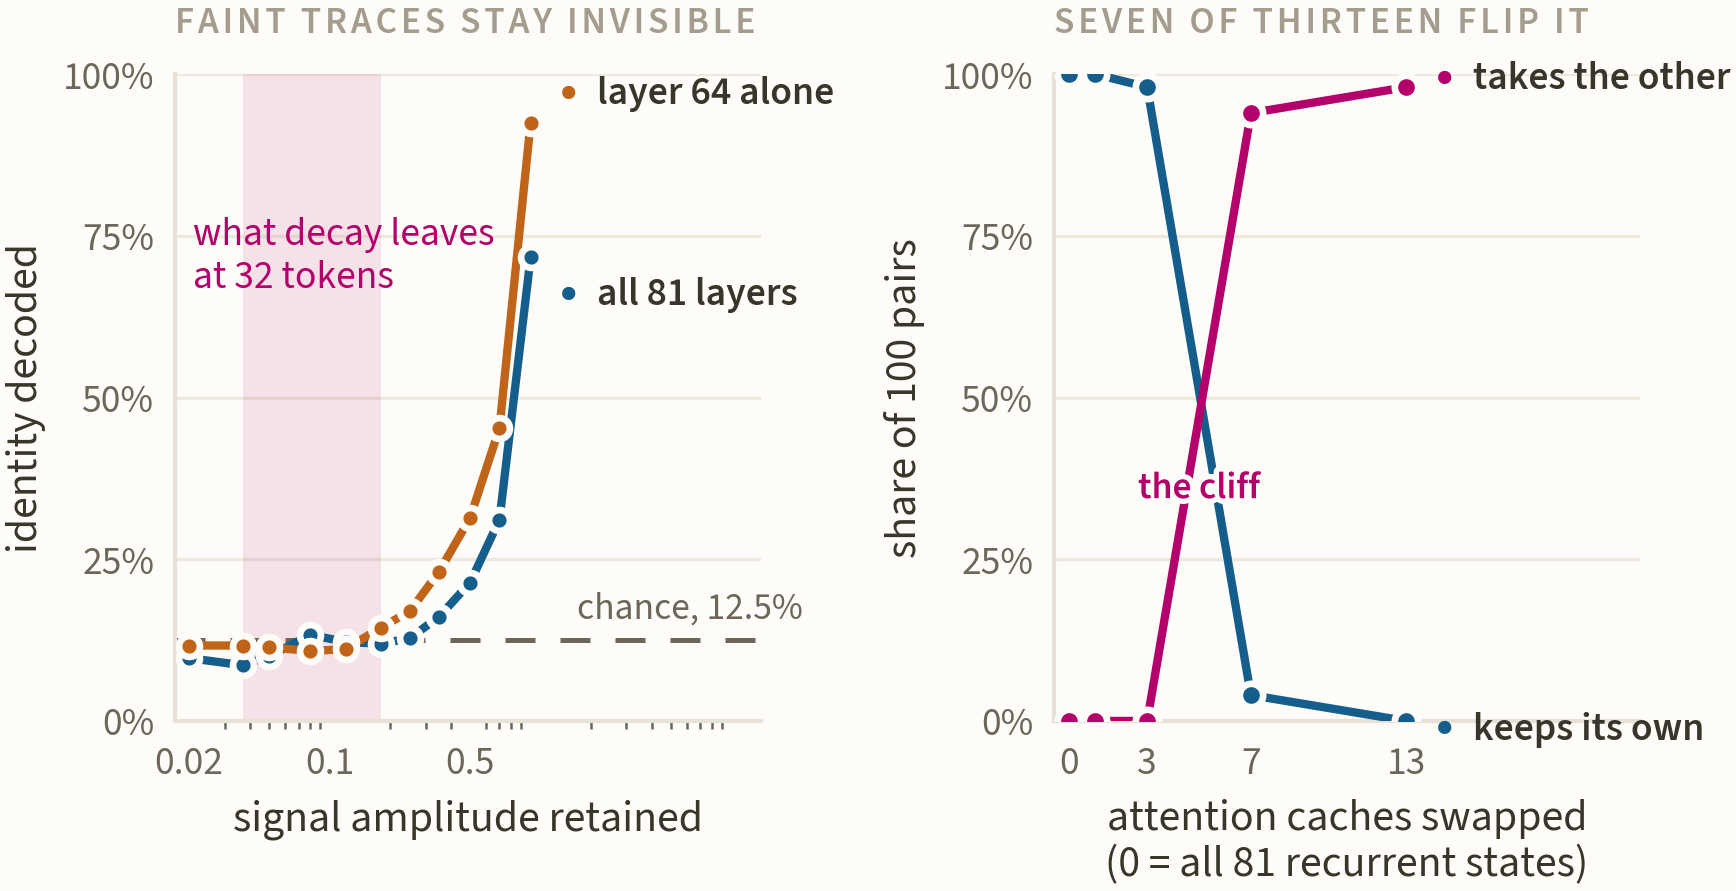
\includegraphics[width=\linewidth]{assets/f7_sens_splice.png}
\caption{\textbf{Left:} how faint a signal the probe can still recover. The
shaded band is what the model's decay parameters leave of a stored trace after
32 tokens, between the median and the mean over heads. Both probes are at chance
throughout that band, so a visible reading at 32 tokens cannot be a retained
one. \textbf{Right:} how many of the thirteen attention caches must be exchanged
before the answer follows the other image, over 100 pairs in which both images
were answered correctly beforehand. The leftmost point is the recurrent swap:
all 81 states replaced, no attention cache touched, no effect.}
\label{fig:sens_splice}
\end{figure}

\section{Causally, the Answer Follows the Attention Channel}
\label{sec:splice}

The probe results say the attention channel supplies what the recurrent state
appears to hold. The splice tests the same claim on the model's own behaviour,
with no probe involved. Two runs see different images, one memory channel is
exchanged between them, and the host run then answers its question. We admit a
pair only if host and donor each answered their own question correctly
beforehand, so the ceiling is $100\%$ by construction. Of 111 attempted pairs,
11 were rejected on that criterion and none for mismatched cache length. Every
recurrent swap was verified to have changed the state, 100 of 100.

\begin{table}[t]
\centering\small
\begin{tabular}{lrrr}
\toprule
condition & layers swapped & follows host & follows donor \\
\midrule
no swap                       & 0  & $100/100$ $[96,100]$ & $0/100$ $[0,4]$ \\
recurrent, all 81 states      & 0  & $100/100$ $[96,100]$ & $0/100$ $[0,4]$ \\
\addlinespace
attention, 1 layer            & 1  & $100/100$ $[96,100]$ & $0/100$ $[0,4]$ \\
attention, 3 layers spread    & 3  & $98/100$ $[93,99]$   & $0/100$ $[0,4]$ \\
attention, 7 layers           & 7  & $4/100$ $[2,10]$     & $94/100$ $[88,97]$ \\
attention, all 13             & 13 & $0/100$ $[0,4]$      & $98/100$ $[93,99]$ \\
\addlinespace
attention, earliest 3         & 3  & $94/100$ $[88,97]$   & $1/100$ $[0,5]$ \\
attention, latest 3           & 3  & $100/100$ $[96,100]$ & $0/100$ $[0,4]$ \\
both channels                 & 13 & $0/100$ $[0,4]$      & $100/100$ $[96,100]$ \\
\bottomrule
\end{tabular}
\caption{The splice at 100 pairs with a $100\%$ ceiling. Brackets are $95\%$
Wilson intervals in percent. Replacing the entire recurrent memory of all 81
layers changes nothing; replacing seven of the thirteen attention caches flips
the answer to the other image.}
\label{tab:splice}
\end{table}

Three things can be read from the table. First, replacing the recurrent memory
has no effect at all: exchanging all 81 states leaves $100$ of $100$ answers
following the host's own image. Second, the attention channel is causally
sufficient to determine the
answer: swapping seven of the thirteen caches moves $94$ of $100$ answers to
the donor's image. Third, the dependence on attention is graded and
distributed. One swapped layer changes nothing, three spread across the stack
move two answers, and seven move almost all of them, so the picture is held
across the attention layers rather than concentrated in a few. The earliest
three layers matter where the latest three do not, which matches the layerwise
eviction of Section~\ref{sec:controls}.

Why does replacing the entire recurrent memory change nothing? The relay
result already answers this. The transplanted state is decayed away within a
few tokens and rewritten from the attention channel, which the recurrent swap
leaves untouched. The probe result and the splice result are the same fact
seen from two sides.

\section{Scale, and Where the Prediction Fails}
\label{sec:scale}

We repeated the core protocol at three model scales. The instruments read
every tensor shape from the loaded model's configuration rather than assuming
the 7B geometry. This is a requirement, not a convenience: the 2.7B and 1.2B
checkpoints use a single B/C group where the 7B uses two, and the 1.2B has a
state dimension of 128 where the others have 64.

\begin{table}[t]
\centering\small
\begin{tabular}{lrrrrrr}
\toprule
model & layers & attn & probe $d{=}0$ & probe $d{=}64$ & measured $t_{1/2}$ & predicted $t_{1/2}$ \\
\midrule
Zamba2-VL-7B   & 81 & 13 & $71.7\%$ & $21.7\%$ & $4.0$  & $6.64$ \\
Zamba2-VL-2.7B & 54 &  9 & $84.2\%$ & $31.7\%$ & $9.6$  & $2.91$ \\
Zamba2-VL-1.2B & 38 &  6 & $83.3\%$ & $34.2\%$ & $14.3$ & $2.58$ \\
\bottomrule
\end{tabular}
\caption{The same protocol at three scales, 120 identity trials per distance.
The pre-image control reads exactly $12.5\%$ at every scale. Half-lives are in
tokens: measured is the distance at which above-chance decodability halves,
predicted is the median over heads of $\ln 2/(|A|\bar{\Delta})$.}
\label{tab:scale}
\end{table}

Two conclusions follow, and the second is a negative result we report plainly.
First, the parameter-derived horizon is short at every scale: median predicted
half-lives are $6.64$, $2.91$ and $2.58$ tokens, with $85.0\%$, $97.9\%$ and
$95.6\%$ of heads under 32 tokens. Second, the predicted horizon does not
predict the measured one. Across the three models the two quantities move in
opposite directions: the prediction falls with scale while the measurement
rises. The $r = 0.973$ agreement on the 7B does not replicate, so we do not
claim the decay calculation explains the measured decay curve.
Section~\ref{sec:relay} shows why it cannot: the probe at distance was never
measuring retention in the first place.

\section{Visual Key-Value Eviction Removes the Only Copy, Eventually}
\label{sec:eviction}

Pruning methods discard visual key-value entries on the premise that they are
redundant. Our results say the redundancy comes from the relay, and the relay
is short-lived, so the premise should degrade with distance. We test this
directly on the model's own behaviour. We evict a fraction of the visual
key-value entries from all 13 attention layers immediately after the image is
read, let the filler and the question stream past the pruned cache, and
measure the model's accuracy. Retention $\rho$ is the fraction of visual
positions kept, sampled uniformly, and the question is asked $d$ tokens after
the image.

\begin{table}[t]
\centering\small
\begin{tabular}{lrrrr}
\toprule
visual KV retained & $d{=}0$ & $d{=}32$ & $d{=}128$ & $d{=}512$ \\
\midrule
$100\%$ & $97.9\%$ & $95.8\%$ & $100.0\%$ & $97.9\%$ \\
$25\%$  & $91.7\%$ & $95.8\%$ & $95.8\%$  & $91.7\%$ \\
$5\%$   & $87.5\%$ & $77.1\%$ & $75.0\%$  & $64.6\%$ \\
$0\%$   & $64.6\%$ & $37.5\%$ & $31.2\%$  & $22.9\%$ \\
\bottomrule
\end{tabular}
\caption{Behavioural accuracy under visual key-value eviction, against distance
between the image and the question. $n = 48$ per cell, chance $12.5\%$, no
failures. The unpruned row is flat, so distance alone costs nothing.}
\label{tab:eviction}
\end{table}

With a quarter of the entries retained there is no distance effect at all. The
cost relative to the unpruned baseline at the same distance is $6.2$, $0.0$,
$4.2$ and $6.2$ points, flat within noise. At that level the redundancy
premise holds on this architecture, and we found no evidence against it. Below
that level distance matters a great deal. At a twentieth retained the cost
triples across the range, from $10.4$ points beside the image to $33.3$ at 512
tokens; with every visual entry removed it runs from $33.3$ to $75.0$
(Table~\ref{tab:eviction_cost}, appendix). The unpruned row is flat across the
same distances, so long prompts are not hard in themselves. They become hard
\emph{once the visual entries are gone}, because by then the recurrent channel
has nothing left to relay from. The cost of heavy pruning is therefore not
one number. Above a retention threshold, here between a quarter and a
twentieth, pruning costs the same at every distance; below it, the cost grows
with distance, and a method validated at short range understates its
long-range cost threefold at $5\%$ retention.

The zero-retention row measures what the recurrent channel contributes on its
own. With no visual entries anywhere in the caches, the model can only be
answering from its recurrent states, and its accuracy falls from $64.6\%$
beside the image to $22.9\%$ at 512 tokens. This is a behavioural measurement,
independent of the probe, and it agrees with the picture the probe gives. One
discrepancy is worth stating plainly. At zero retention the model still
answers at $37.5\%$ at thirty-two tokens while the probe reads the state near
chance, so the model is using something the probe does not recover. The probe
is a lower bound, and our evidence does not support the sentence ``the state
is empty''.

\section{Limitations}

\textbf{The probe is a lower bound, and our own behavioural data prove it.}
With every visual key-value entry removed, the model answers at $37.5\%$ at
thirty-two tokens while the probe reads near chance. Every statement here
about what the state contains is therefore a statement about what is linearly
decodable under this instrument. Accuracies are comparable only within a
collection: the full $41{,}472$-dimensional probe reads $71.7\%$ where one
layer's 512 features read $92.5\%$ on identical trials.

\textbf{A sensitivity asymmetry is bounded but not eliminated.}
Section~\ref{sec:sensitivity} calibrates the detection floor and shows that a
visible reading at thirty-two tokens cannot be a retained one. That argument
assumes decay followed by overwriting acts on the discriminative component
roughly as our attenuation does. A model with no attention channel to relay
from would settle the question without that assumption, and we have not tested
one. Relatedly, the route is located but not traced: visual information enters
early, but the path from attention output through the residual stream into a
downstream mixer's write is not followed.

\textbf{The dose-response is confirmed at matched amplitude only at distance
zero.} Every split by half-life is also a split by write amplitude. With the
gate held fixed, the eviction dose-response is a $2.4\times$ ratio over two
strata at one distance ($n = 192$ per cell). At thirty-two tokens the
gain-matched fast stratum reads too close to chance even when intact for the
contrast to be informative. Two strata at one distance in one model is a
direction, not a curve.

\textbf{One model family, and a second family we tried and failed on.} Results
come from three Zamba2-VL checkpoints: one vendor, one architecture family,
one training recipe. This is the principal limit on generality. We attempted
to extend the relay result to Granite 4.0 h-tiny \citep{granite4}, a Mamba2
hybrid from a different lineage. The horizon calculation transfers cleanly
(median predicted half-life $8.7$ tokens). The relay contrast does not,
because the probe reads that model's recurrent state at chance even at
distance zero, on a task it answers at $100\%$ (Appendix~\ref{app:granite}).
We do not know why the instrument fails there, so no relay claim can be made
beyond the Zamba2-VL family on this evidence. The sharper test remains a
vision-language model with no attention layers at all, such as Cobra
\citep{zhao2025cobra} or VL-Mamba \citep{qiao2024vlmamba}; both are Mamba1
models and would need the read operator ported first.

\textbf{One task format, one dataset, one filler distribution.} Eight-way
forced choice on COCO buys an exact chance rate and a clean pre-image control.
It costs generality to free-form answering and to other visual properties.
$\bar{\Delta}$ is input dependent: measured on natural prose, the median
half-life is stable across images ($6.44$ to $6.86$ tokens), but a filler with
very different gate statistics would give a different horizon, which the same
calculation predicts.

\section{Conclusion}

The recurrent state of this hybrid vision-language model is not a memory of
the image in any useful sense. It is a selective summary of the picture's
gist, and it holds that summary for only about four tokens. That lifetime can
be computed from the model's own decay parameters before any measurement is
taken. What the model answers from lives in the thin attention channel. The
practical consequence is direct: the visual key-value entries a hybrid carries
are redundant only for as long as the recurrent state is still relaying the
picture, and that is not long.

\section*{Reproducibility Statement}

Every number in this paper comes from a scripted experiment against public
checkpoints on public data. The model is Zamba2-VL-7B \citep{zamba2vl} together
with its 2.7B and 1.2B siblings, all Apache-2.0; trials are built from COCO
val2017 annotations \citep{lin2014coco}. Section 3 gives the recurrence, the
projection width, the probe and its cross-validation scheme, and the exact
statistical tests; the decay prediction is stated in closed form in Section 5
with $\bar{\Delta}$ measured as described. The instruments read layer counts,
head counts, group counts and state widths from each loaded checkpoint's own
configuration rather than assuming the 7B geometry, which is what let the same
code run at three scales and on a second family. Appendix~\ref{app:tables}
reports the full tables behind the summarised results, including the fine
distance sweep, the per-decile control values and the seed repeats. Source for
the instruments, the analysis and the figures accompanies the submission.

\section*{Ethics Statement}

This work analyses publicly released model checkpoints on a public image
dataset, involves no human subjects and collects no new data. COCO images depict
people, and our trials ask only about object category, count and position; no
attribute inference about depicted persons is performed. The interpretability
findings are dual-use in the ordinary sense that understanding where a model
holds information could inform both better and worse systems, but they identify
no vulnerability and enable no capability that inspection of the open weights
would not. We report a negative result rather than omitting it.

\section*{Use of Large Language Models}

Large language models were used as coding and writing assistants: drafting and
refactoring experiment and analysis code, and copy-editing prose. All
experimental design, all interpretation of results, and all claims in this paper
are the authors'. Every number reported was produced by the scripted pipeline
and checked against its source output; no text describing results was accepted
without that check.

\bibliographystyle{iclr2026_conference}
\begin{thebibliography}{99}\small\setlength{\itemsep}{1pt}

\bibitem[Alain \& Bengio(2016)]{alain2016probes}
G.~Alain and Y.~Bengio.
\newblock Understanding Intermediate Layers Using Linear Classifier Probes.
\emph{arXiv:1610.01644}, 2016.

\bibitem[Arora et al.(2023)]{arora2023zoology}
S.~Arora, S.~Eyuboglu, A.~Timalsina, I.~Johnson, M.~Poli, J.~Zou, A.~Rudra,
and C.~R\'e.
\newblock Zoology: Measuring and Improving Recall in Efficient Language Models.
\emph{arXiv:2312.04927}, 2023.

\bibitem[Arora et al.(2024)]{arora2024based}
S.~Arora, S.~Eyuboglu, M.~Zhang, A.~Timalsina, S.~Alberti, D.~Zinsley, J.~Zou,
A.~Rudra, and C.~R\'e.
\newblock Simple Linear Attention Language Models Balance the Recall-Throughput
Tradeoff. \emph{arXiv:2402.18668}, 2024.

\bibitem[Bai et al.(2025)]{bai2025qwen25vl}
S.~Bai, K.~Chen, X.~Liu, J.~Wang, W.~Ge, S.~Song, et~al.
\newblock Qwen2.5-VL Technical Report. \emph{arXiv:2502.13923}, 2025.

\bibitem[Beck et al.(2024)]{beck2024xlstm}
M.~Beck, K.~P\"oppel, M.~Spanring, A.~Auer, O.~Prudnikova, M.~Kopp,
G.~Klambauer, J.~Brandstetter, and S.~Hochreiter.
\newblock xLSTM: Extended Long Short-Term Memory.
\emph{arXiv:2405.04517}, 2024.

\bibitem[Belinkov(2022)]{belinkov2022probing}
Y.~Belinkov.
\newblock Probing Classifiers: Promises, Shortcomings, and Advances.
\emph{Computational Linguistics}, 2022.

\bibitem[Chen et al.(2024)]{chen2024fastv}
L.~Chen, H.~Zhao, T.~Liu, S.~Bai, J.~Lin, C.~Zhou, and B.~Chang.
\newblock An Image is Worth 1/2 Tokens After Layer 2: Plug-and-Play Inference
Acceleration for Large Vision-Language Models. \emph{ECCV}, 2024.

\bibitem[Dao \& Gu(2024)]{dao2024mamba2}
T.~Dao and A.~Gu.
\newblock Transformers are SSMs: Generalized Models and Efficient Algorithms
Through Structured State Space Duality. \emph{ICML}, 2024.

\bibitem[De et al.(2024)]{de2024griffin}
S.~De, S.~L. Smith, A.~Fernando, A.~Botev, G.~Cristian-Muraru, A.~Gu, et~al.
\newblock Griffin: Mixing Gated Linear Recurrences with Local Attention for
Efficient Language Models. \emph{arXiv:2402.19427}, 2024.

\bibitem[Glorioso et al.(2024)]{glorioso2024zamba}
P.~Glorioso, Q.~Anthony, Y.~Tokpanov, J.~Whittington, J.~Pilault, A.~Ibrahim,
and B.~Millidge.
\newblock Zamba: A Compact 7B SSM Hybrid Model.
\emph{arXiv:2405.16712}, 2024.

\bibitem[Gu \& Dao(2023)]{gu2023mamba}
A.~Gu and T.~Dao.
\newblock Mamba: Linear-Time Sequence Modeling with Selective State Spaces.
\emph{arXiv:2312.00752}, 2023.

\bibitem[Gu et al.(2022)]{gu2022s4}
A.~Gu, K.~Goel, and C.~R\'e.
\newblock Efficiently Modeling Long Sequences with Structured State Spaces.
\emph{ICLR}, 2022.

\bibitem[Hewitt \& Liang(2019)]{hewitt2019control}
J.~Hewitt and P.~Liang.
\newblock Designing and Interpreting Probes with Control Tasks.
\emph{EMNLP}, 2019.

\bibitem[IBM Granite Team(2025)]{granite4}
IBM Granite Team.
\newblock Granite 4.0 h-tiny model card.
\newblock \url{https://huggingface.co/ibm-granite/granite-4.0-h-tiny}, 2025.

\bibitem[Jelassi et al.(2024)]{jelassi2024copying}
S.~Jelassi, D.~Brandfonbrener, S.~M. Kakade, and E.~Malach.
\newblock Repeat After Me: Transformers are Better than State Space Models at
Copying. \emph{arXiv:2402.01032}, 2024.

\bibitem[Katharopoulos et al.(2020)]{katharopoulos2020linear}
A.~Katharopoulos, A.~Vyas, N.~Pappas, and F.~Fleuret.
\newblock Transformers are RNNs: Fast Autoregressive Transformers with Linear
Attention. \emph{ICML}, 2020.

\bibitem[Li et al.(2024)]{li2024snapkv}
Y.~Li, Y.~Huang, B.~Yang, B.~Venkitesh, A.~Locatelli, H.~Ye, T.~Cai, P.~Lewis,
and D.~Chen.
\newblock SnapKV: LLM Knows What You are Looking for Before Generation.
\emph{arXiv:2404.14469}, 2024.

\bibitem[Lieber et al.(2024)]{lieber2024jamba}
O.~Lieber, B.~Lenz, H.~Bata, G.~Cohen, J.~Osin, I.~Dalmedigos, et~al.
\newblock Jamba: A Hybrid Transformer-Mamba Language Model.
\emph{arXiv:2403.19887}, 2024.

\bibitem[Lin et al.(2014)]{lin2014coco}
T.-Y. Lin, M.~Maire, S.~Belongie, L.~Bourdev, R.~Girshick, J.~Hays, P.~Perona,
D.~Ramanan, C.~L. Zitnick, and P.~Doll\'ar.
\newblock Microsoft COCO: Common Objects in Context.
\newblock \emph{ECCV}, 2014. arXiv:1405.0312.

\bibitem[Liu et al.(2023)]{liu2023llava}
H.~Liu, C.~Li, Q.~Wu, and Y.~J. Lee.
\newblock Visual Instruction Tuning. \emph{NeurIPS}, 2023.

\bibitem[Meng et al.(2022)]{meng2022rome}
K.~Meng, D.~Bau, A.~Andonian, and Y.~Belinkov.
\newblock Locating and Editing Factual Associations in GPT.
\emph{NeurIPS}, 2022.

\bibitem[Merrill et al.(2024)]{merrill2024illusion}
W.~Merrill, J.~Petty, and A.~Sabharwal.
\newblock The Illusion of State in State-Space Models. \emph{ICML}, 2024.

\bibitem[Peng et al.(2023)]{peng2023rwkv}
B.~Peng, E.~Alcaide, Q.~Anthony, A.~Albalak, S.~Arcadinho, S.~Biderman, et~al.
\newblock RWKV: Reinventing RNNs for the Transformer Era.
\emph{arXiv:2305.13048}, 2023.

\bibitem[Qiao et al.(2024)]{qiao2024vlmamba}
Y.~Qiao, Z.~Yu, L.~Guo, S.~Chen, Z.~Zhao, M.~Sun, Q.~Wu, and J.~Liu.
\newblock VL-Mamba: Exploring State Space Models for Multimodal Learning.
\emph{arXiv:2403.13600}, 2024.

\bibitem[Ren et al.(2025)]{ren2025samba}
L.~Ren, Y.~Liu, Y.~Lu, Y.~Shen, C.~Liang, and W.~Chen.
\newblock Samba: Simple Hybrid State Space Models for Efficient Unlimited
Context Language Modeling. \emph{ICLR}, 2025.

\bibitem[Shang et al.(2025)]{shang2025prumerge}
Y.~Shang, M.~Cai, B.~Xu, Y.~J. Lee, and Y.~Yan.
\newblock LLaVA-PruMerge: Adaptive Token Reduction for Efficient Large
Multimodal Models. \emph{ICCV}, 2025.

\bibitem[Vig et al.(2020)]{vig2020causal}
J.~Vig, S.~Gehrmann, Y.~Belinkov, S.~Qian, D.~Nevo, S.~Sakenis, J.~Huang,
Y.~Singer, and S.~Shieber.
\newblock Causal Mediation Analysis for Interpreting Neural NLP: The Case of
Gender Bias. \emph{arXiv:2004.12265}, 2020.

\bibitem[Waleffe et al.(2024)]{waleffe2024empirical}
R.~Waleffe, W.~Byeon, D.~Riach, B.~Norick, V.~Korthikanti, T.~Dao, A.~Gu,
et~al.
\newblock An Empirical Study of Mamba-based Language Models.
\emph{arXiv:2406.07887}, 2024.

\bibitem[Wang et al.(2022)]{wang2022ioi}
K.~Wang, A.~Variengien, A.~Conmy, B.~Shlegeris, and J.~Steinhardt.
\newblock Interpretability in the Wild: a Circuit for Indirect Object
Identification in GPT-2 small. \emph{arXiv:2211.00593}, 2022.

\bibitem[Wen et al.(2024)]{wen2024rnns}
K.~Wen, X.~Dang, and K.~Lyu.
\newblock RNNs are not Transformers (Yet): The Key Bottleneck on In-context
Retrieval. \emph{arXiv:2402.18510}, 2024.

\bibitem[Xiao et al.(2024)]{xiao2024streaming}
G.~Xiao, Y.~Tian, B.~Chen, S.~Han, and M.~Lewis.
\newblock Efficient Streaming Language Models with Attention Sinks.
\emph{ICLR}, 2024.

\bibitem[Yang et al.(2024)]{yang2024visionzip}
S.~Yang, Y.~Chen, Z.~Tian, C.~Wang, J.~Li, B.~Yu, and J.~Jia.
\newblock VisionZip: Longer is Better but Not Necessary in Vision Language
Models. \emph{arXiv:2412.04467}, 2024.

\bibitem[Zhang \& Nanda(2024)]{zhang2024patching}
F.~Zhang and N.~Nanda.
\newblock Towards Best Practices of Activation Patching in Language Models:
Metrics and Methods. \emph{ICLR}, 2024.

\bibitem[Zhang et al.(2023)]{zhang2023h2o}
Z.~Zhang, Y.~Sheng, T.~Zhou, T.~Chen, L.~Zheng, R.~Cai, Z.~Song, Y.~Tian,
C.~R\'e, C.~Barrett, Z.~Wang, and B.~Chen.
\newblock H\textsubscript{2}O: Heavy-Hitter Oracle for Efficient Generative
Inference of Large Language Models. \emph{arXiv:2306.14048}, 2023.

\bibitem[Zhao et al.(2025)]{zhao2025cobra}
H.~Zhao, M.~Zhang, W.~Zhao, P.~Ding, S.~Huang, and D.~Wang.
\newblock Cobra: Extending Mamba to Multi-Modal Large Language Model for
Efficient Inference. \emph{AAAI}, 2025.

\bibitem[Zyphra(2026)]{zamba2vl}
Zyphra.
\newblock Zamba2-VL-7B model card.
\newblock \url{https://huggingface.co/Zyphra/Zamba2-VL-7B}, 2026. Apache-2.0.

\end{thebibliography}

\appendix

\section{Full Tables}
\label{app:tables}

This appendix carries the tables behind the summarised results in the body: the
fine distance sweep, the matched-eviction control in full by decile, the seed
repeat of the eviction contrast, and the pruning costs relative to the unpruned
baseline at each distance. Cell counts and chance rates are stated in each
caption.

\begin{table}[h]
\centering\small
\begin{tabular}{rrrrr}
\toprule
tokens & probe accuracy & $p$ & behaviour & predicted retention (median) \\
\midrule
0  & $71.7\%$ & $2\times10^{-50}$ & $94.2\%$ & $1.000$ \\
1  & $60.0\%$ & $2\times10^{-34}$ & $96.7\%$ & $0.901$ \\
2  & $59.2\%$ & $2\times10^{-33}$ & $97.5\%$ & $0.812$ \\
4  & $41.7\%$ & $1\times10^{-15}$ & $96.7\%$ & $0.659$ \\
8  & $35.0\%$ & $2\times10^{-10}$ & $97.5\%$ & $0.434$ \\
12 & $30.0\%$ & $3\times10^{-7}$  & $96.7\%$ & $0.286$ \\
16 & $24.2\%$ & $3\times10^{-4}$  & $97.5\%$ & $0.188$ \\
24 & $29.2\%$ & $1\times10^{-6}$  & $95.8\%$ & $0.082$ \\
32 & $20.8\%$ & $7\times10^{-3}$  & $95.0\%$ & $0.036$ \\
48 & $25.8\%$ & $6\times10^{-5}$  & $97.5\%$ & $0.007$ \\
64 & $21.7\%$ & $3\times10^{-3}$  & $98.3\%$ & $0.001$ \\
\bottomrule
\end{tabular}
\caption{The fine distance sweep of Section~\ref{sec:horizon}: decodability of
object identity against distance from the image, 120 trials at every distance,
with the retention predicted from the weights alongside. Chance is $12.5\%$; the
pre-image control reads exactly $12.5\%$. Beyond 16 tokens the measured curve
sits between the predicted median and mean, which is what the heavy tail of slow
heads predicts.}
\label{tab:fine}
\end{table}

\begin{table}[h]
\centering\small
\begin{tabular}{p{0.44\linewidth}p{0.48\linewidth}}
\toprule
\textbf{Established by prior work} & \textbf{New here} \\
\midrule
A fixed-size state must lose information from context, with a capacity proof
and behavioural evidence \citep{jelassi2024copying,merrill2024illusion,wen2024rnns}.
& \emph{When}. A retention horizon in tokens, computed from the model's own
$A$ and $\Delta$ with nothing fitted, at three scales. \\
\addlinespace
Recurrent models underperform at copying and retrieval as a class
\citep{arora2023zoology,arora2024based}.
& \emph{What survives}. The failure is content-selective: object identity is
highly decodable at the same instant that count and position are near chance. \\
\addlinespace
Architectures are compared to one another from the outside.
& \emph{Causal localisation inside one model}, and the finding that the
recurrent channel relays rather than stores, which makes probing it at distance
a measurement of the attention channel. \\
\addlinespace
Visual tokens and key-value entries carry substantial redundancy that can be
pruned \citep{chen2024fastv,yang2024visionzip,shang2025prumerge}.
& \emph{What underwrites that premise}, and that its safety margin shrinks
with distance from the image on a hybrid. \\
\bottomrule
\end{tabular}
\caption{Delineation of prior work and contribution.}
\label{tab:novelty}
\end{table}

\begin{table}[h]
\centering\small
\begin{tabular}{lrrrrr}
\toprule
& \multicolumn{2}{c}{fastest decile ($t_{1/2} = 0.7$)} & \multicolumn{3}{c}{mean over ten deciles} \\
\cmidrule(lr){2-3}\cmidrule(lr){4-6}
condition & $d{=}0$ & $d{=}32$ & $d{=}0$ & $d{=}32$ & effect \\
\midrule
no eviction               & $56.2\%$ & $31.2\%$ & $44.2\%$ & $20.5\%$ & baseline \\
evict image               & $18.8\%$ & $12.5\%$ & $25.5\%$ & $14.1\%$ & $-18.7$, $-6.4$ \\
evict matched text        & $78.1\%$ & $60.9\%$ & $58.9\%$ & $33.0\%$ & $+14.7$, $+12.5$ \\
\bottomrule
\end{tabular}
\caption{The matched control, $n = 64$ per cell, chance $12.5\%$. Both
interventions delete the same number of positions from the same 13 caches, one
taking the image and one an equal count of the most recent pre-image text. They
move the readout in opposite directions, which a perturbation account cannot
produce. The last column gives the mean effect in points at $d{=}0$ and
$d{=}32$.}
\label{tab:controls}
\end{table}

\begin{table}[h]
\centering\small
\begin{tabular}{rrrrrrr}
\toprule
& & \multicolumn{3}{c}{$d = 0$} & \multicolumn{2}{c}{$d = 32$} \\
\cmidrule(lr){3-5}\cmidrule(lr){6-7}
decile & pred.\ $t_{1/2}$ & intact & evict image & evict text & intact & evict image \\
\midrule
1  & $0.70$ & $56.2\%$ & $18.8\%$ & $78.1\%$ & $31.2\%$ & $12.5\%$ \\
2  & $1.84$ & $56.2\%$ & $17.2\%$ & $79.7\%$ & $29.7\%$ & $12.5\%$ \\
3  & $2.75$ & $53.1\%$ & $18.8\%$ & $73.4\%$ & $20.3\%$ & $4.7\%$  \\
4  & $3.79$ & $46.9\%$ & $21.9\%$ & $71.9\%$ & $23.4\%$ & $15.6\%$ \\
5  & $5.38$ & $31.2\%$ & $26.6\%$ & $42.2\%$ & $12.5\%$ & $9.4\%$  \\
6  & $8.15$ & $35.9\%$ & $40.6\%$ & $51.6\%$ & $17.2\%$ & $20.3\%$ \\
7  & $11.8$ & $37.5\%$ & $25.0\%$ & $54.7\%$ & $10.9\%$ & $9.4\%$  \\
8  & $17.8$ & $45.3\%$ & $29.7\%$ & $57.8\%$ & $20.3\%$ & $18.8\%$ \\
9  & $32.0$ & $28.1\%$ & $26.6\%$ & $32.8\%$ & $15.6\%$ & $15.6\%$ \\
10 & $73.3$ & $51.6\%$ & $29.7\%$ & $46.9\%$ & $23.4\%$ & $21.9\%$ \\
\bottomrule
\end{tabular}
\caption{The matched-eviction control of Section~\ref{sec:controls} in full, by
decile of predicted half-life, $n = 64$ per cell, chance $12.5\%$. ``Evict
image'' and ``evict text'' delete the same number of positions from the same 13
attention caches. Single cells carry about $6$ points of binomial noise at
$n = 64$, and two of the twenty image-eviction cells fall slightly the wrong
way; the trend rather than any one cell is the result. The drop under image
eviction correlates with the decay rate $1/t_{1/2}$ at $r = 0.647$ at $d{=}0$
and $r = 0.800$ at $d{=}32$.}
\label{tab:controls_full}
\end{table}

\begin{table}[h]
\centering\small
\begin{tabular}{llrrr}
\toprule
stratum & condition & seed 0 & seed 1 & seed 2 \\
\midrule
fast   & $d{=}0$, intact       & $62.5\%$ & $64.1\%$ & $64.1\%$ \\
fast   & $d{=}0$, evicted      & $18.8\%$ & $20.3\%$ & $18.8\%$ \\
fast   & $d{=}32$, intact      & $32.8\%$ & $29.7\%$ & $31.2\%$ \\
fast   & $d{=}32$, evicted     & $7.8\%$  & $10.9\%$ & $10.9\%$ \\
\addlinespace
middle & $d{=}32$, intact      & $14.1\%$ & $12.5\%$ & $10.9\%$ \\
middle & $d{=}32$, evicted     & $14.1\%$ & $12.5\%$ & $9.4\%$  \\
\addlinespace
slow   & $d{=}32$, intact      & $12.5\%$ & $15.6\%$ & $17.2\%$ \\
slow   & $d{=}32$, evicted     & $14.1\%$ & $15.6\%$ & $17.2\%$ \\
\bottomrule
\end{tabular}
\caption{The eviction contrast repeated across three independent Gaussian
projection bases, $n = 64$ per cell, chance $12.5\%$. The fast tercile's
dependence on the attention channel is stable across bases (intact
$31.2 \pm 1.6\%$ against evicted $9.9 \pm 1.8\%$ at $d{=}32$, mean and standard
deviation over seeds), while the slow tercile shows no eviction effect at any
seed. The decay-curve collections elsewhere in the paper use a single fixed
basis.}
\label{tab:seeds}
\end{table}

\begin{table}[h]
\centering\small
\begin{tabular}{lrrrr}
\toprule
visual KV retained & $d{=}0$ & $d{=}32$ & $d{=}128$ & $d{=}512$ \\
\midrule
$25\%$ & $6.2$  & $0.0$  & $4.2$  & $6.2$ \\
$5\%$  & $10.4$ & $18.8$ & $25.0$ & $33.3$ \\
$0\%$  & $33.3$ & $58.3$ & $68.8$ & $75.0$ \\
\bottomrule
\end{tabular}
\caption{Accuracy points lost to pruning, relative to the unpruned baseline at
the same distance (Section~\ref{sec:eviction}).}
\label{tab:eviction_cost}
\end{table}

\begin{figure}[h]
\centering
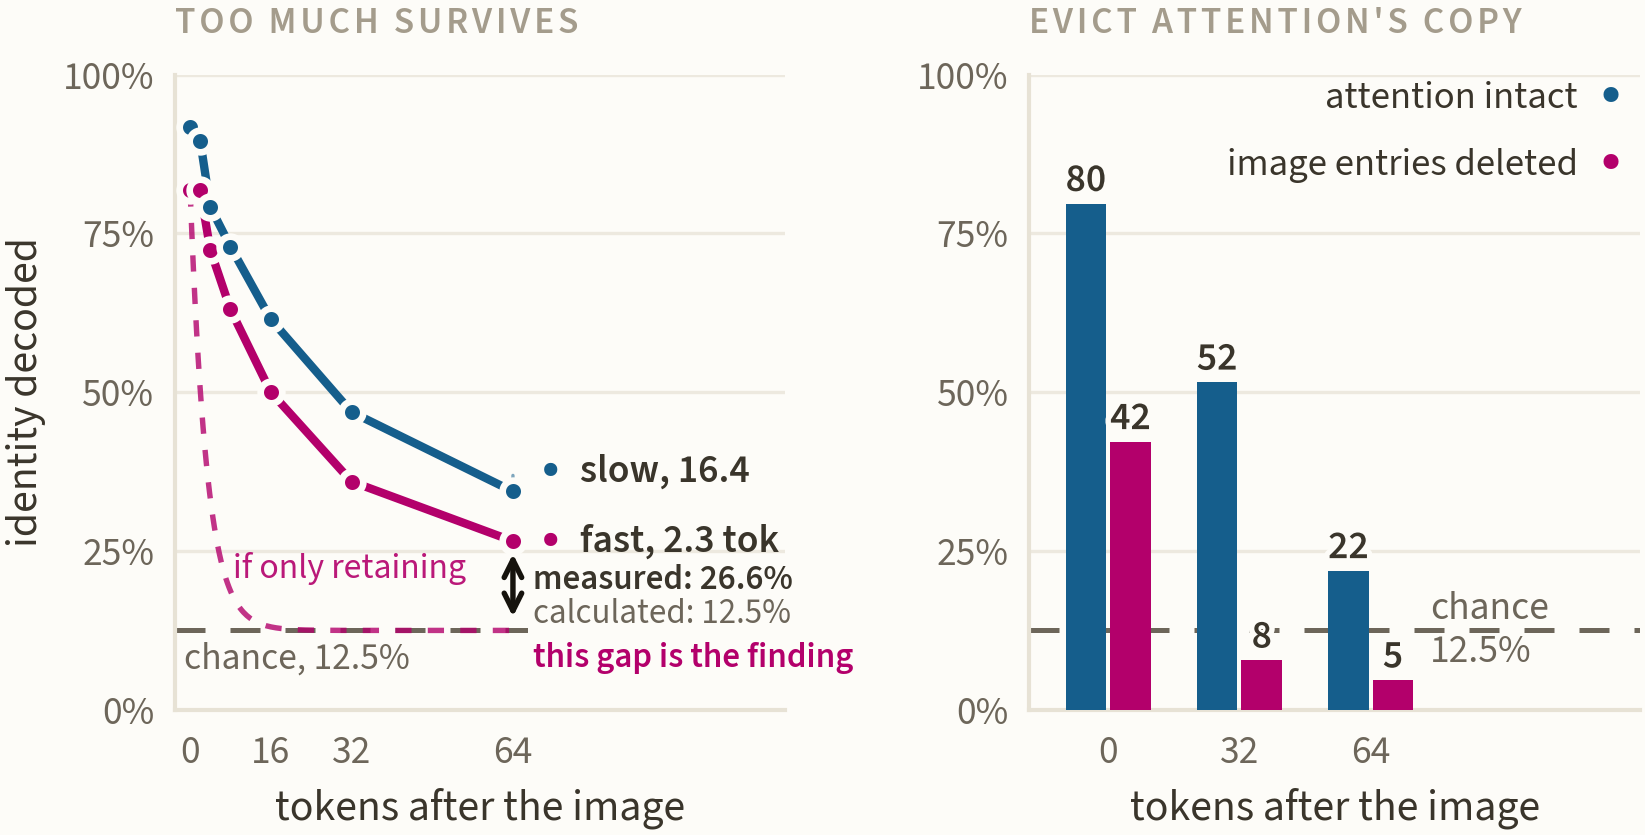
\includegraphics[width=\linewidth]{assets/f2_relay.png}
\caption{\textbf{Left: how to read this panel.} The two solid curves are
measurements: identity decoded from the slow and fast strata at matched write
gain, $n = 192$ per point. The dashed curve is not a measurement but a
calculation: where the fast stratum would read if its signal came only from
what its own $2.3$-token half-life retains. The calculation reaches chance
within ten tokens; the measurement ends at $26.6\%$ at $d{=}64$. The
slow-above-fast ordering is what decay predicts; the gap between the two fast
curves is what decay cannot explain. \textbf{Right:} the same recurrent state
probed with and without the attention channel's copy of the image, fast
tercile, $n = 64$ per bar. The eviction never touches the recurrent state,
which is identical in both runs at that instant.}
\label{fig:relay}
\end{figure}

\begin{figure}[h]
\centering

\includegraphics[width=0.72\linewidth]{assets/f6_eviction.png}
\caption{Model accuracy under visual key-value eviction, against how far the
question sits from the image, $n = 48$ per point. The unpruned line is flat, so
distance alone costs nothing. Keeping a quarter of the entries is also flat.
Below that the lines fan out: the cost of pruning grows with distance only once
the recurrent channel has stopped relaying the picture.}
\label{fig:eviction}
\end{figure}


\section{The Second-Family Attempt in Full}
\label{app:granite}

Granite 4.0 h-tiny \citep{granite4} is a Mamba2 hybrid from a different lineage:
40 decoder layers, of which 36 carry a Mamba2 mixer and 4 carry attention (at
indices 5, 15, 25, 35), 48 heads, state dimension 128, one B/C group. Because
its attention layers carry no mixer at all, the recurrent channel spans only 36
of the 40 layers, which is why the instruments ask each model which layers have
mixers rather than assuming every layer does.

The horizon calculation transfers without modification. Reading $A$ and the gate
channels of its input projection gives a median predicted half-life of $8.7$
tokens, the same single-digit regime as the Zamba2-VL family, so
Section~\ref{sec:horizon} is not specific to one vendor.

The relay contrast did not transfer, for an instrumental reason we were unable
to resolve. Granite is a text model, so the carried item is a code word rather
than an image. On a code-word recall task the model answers correctly on
$100\%$, $96.9\%$ and $100\%$ of trials at $0$, $32$ and $64$ tokens, so the
information is demonstrably in the model. Yet a probe on its recurrent state
reads at chance at distance zero, where the Zamba2-VL probe reads $80$ to
$90\%$. Scaling to 256 trials did not change this ($13.7\%$ against a $12.5\%$
chance rate, $p = 0.31$), and neither did probing single layers, where the best
of 36 reached $19.9\%$.

We suspected the item was too small to write a detectable trace: a one-token
code word against the 345-token image of the main experiments. We tested that by
repeating the carrier sixteen times so the item occupied 192 tokens. It did not
help ($12.0\%$, $17.2\%$ and $10.9\%$ across the three strata). Repetition
lengthens an item without diversifying what it writes, so the state ends up
holding little more than the final repeat, which is not the manipulation we
intended.

We do not know why the instrument fails on this model. Candidate explanations
we cannot currently separate include the narrower recurrent channel, the
different item modality, and a genuine architectural difference in what the
state holds. A vision-language hybrid from a second family, where the item is
a real image and the probe is the same one that works here, remains the right
test and we have not run it.

\end{document}
